\chapter{Fundamentos de flujo en aguas subterráneas}

En este capitulo se abordan los principios básicos de la dinámica del agua subterránea en medios porosos, se hace una revisión de los parámetros y variables que condicionan el movimiento del flujo de agua subterránea, principalmente la carga hidráulica y la conductividad hidráulica que son con los que se trabajara en esta tesis; posteriormente, se describiran a profundidad, se discutirá el significado físico de la carga hidráulica y la distribución geoestadística de la conductividad como una forma de caracterizar la heterogeneidad. Finalmente, se deduce la ecuación de flujo a partir de los conceptos anteriormente desarrollados y la ecuación de continuidad.  


\section{Variables y parámetros hidráulicos}

El movimiento del flujo se ve condicionado tanto por las propiedades del medio como las del fluido, la interacción de estas propiedades y su distribución espacial por toda la zona de estudio nos permiten entender la dinámica del flujo en un medio poroso. El estudio de estas propiedades resulta ser de importancia para conocer aspectos relevantes del medio, que es el resultado de un conjunto de procesos geológicos como las zonas de recarga y descarga de un acuífero dentro de una cuenca sedimentaria. Esta información nos permite conocer las caracteristicas necesarias de un pozo o la trayectoria de un contaminante para un proyecto de remediación.
\\

Para comprender la dinámica de fluidos en un medio poroso, es necesario describir principalmente dos elementos que conforman este sistema físico; la carga hidráulica, variable cuya distribución determina la dirección y magnitud del flujo, y la conductividad hidráulica, parámetro que depende de las propiedades del medio. Ambos elementos son posibles de obtener de forma directa a partir de instrumentos de medición o indirectamente con leyes experimentales que las relacionan entre sí. En esta tesis se hablará en particular del movimiento de flujo con agua como fluido de trabajo, aunque tanto la carga hidráulica como la conductividad hidráulica, son conceptos que pueden generalizarse para todo tipo de fluido. 


\subsection{El experimento de Darcy}

El primer experimento sobre el comportamiento de fluidos en medios porosos se registro por primera vez en 1856 por el hidráulico francés Henry Darcy, su estudio sobre medios porosos llevo al descubrimiento de una ley empírica que relaciona la cantidad de flujo con las propiedades del medio, el área donde el campo de flujo intercepta de forma normal y las diferencias en las medidas de posición del flujo respecto a la longitud del tramo medido, esta ley es también conocida como la ecuación de Darcy que describe el fenomeno físico del movimiento de agua en cualquier medio poroso.
\\

El experimento consiste en la adquisición de un tubo cilindrico cuyo interior fue rellenado con arena representando el material poroso y un par de manométros colocados en la entrada y la salida del cilindro, posteriormente se introdujo un liquido en la entrada y se midieron los cambios del flujo volúmetrico en la salida donde se observaron los parámetros dentro del medio que afectan su comportamiento. Este experimento se repitio en distintas ocasiones cambiando el tamaño de grano de la arena, el tipo de fluido y variando la orientación y posición del cilindro, obteniendo diferentes resultados en cada uno de los experimentos (Toth,2009) \cite{Toth2009}.


\begin{figure}[ht!]
\centering
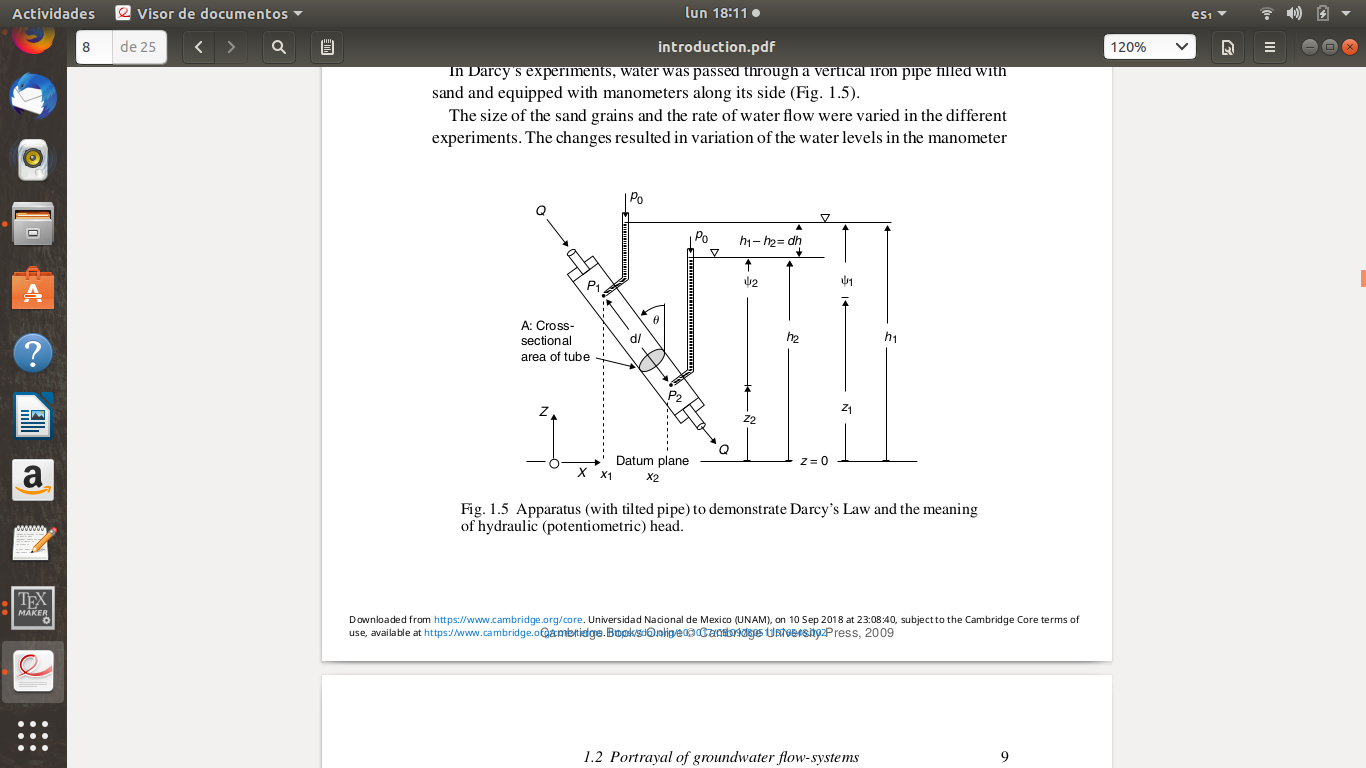
\includegraphics[scale=0.70]{Figura1.png}
\caption{Esquematización del experimento de Darcy (Toth, 2009).}
\label{Figura1:1.1} 
\end{figure}

A partir del esquema del experimento (figura \ref{Figura1:1.1}) podemos observar la presencia de manométros que miden la presión en la entrada y salida del cilindro ($P_{1}$ y $P_{2}$) que conectan con la presión atmosférica $P_{0}$, la presión que existe en esos puntos es proporcional a altura de la columna de fluido representada por $\psi$ (presión de carga), mientras que la altura de los puntos de medición $P_{1}$ y $P_{2}$ desde un dato de referencia $z=0$ se representa con $z_{1}$ y $z_{2}$; Darcy con este experimento encontró que el flujo volumétrico era directamente proporcional al área transversal del cilindro y a partir del estudio de los manómetros instalados, se dio cuenta que el flujo también era directamente proporcional a la diferencia de la altura de los puntos de medición más la altura de la columna del fluido en el manométro medida a partir de un datum de referencia respecto a la longitud entre la posición del fluido en el medio poroso, esta suma le llamó carga hidráulica donde tanto en la Figura \ref{Figura1:1.1} como en la literatura se ve representada como $h$. En casos prácticos se toma como nivel de referencia el nivel del mar aunque puede asumir cualquier valor. La influencia de las propiedades del medio y del fluido, se concentran en la constante de proporcionalidad \textit{K} también conocida como conductividad hidráulica, que supone valores bajos para sedimentos finos como arcillas y valores altos para arenas y gravas. Las ideas anteriores se pueden resumir en la siguiente expresión, llamada ecuación de Darcy:

\begin{equation}
\label{eqn:1.1}
 Q=-KA\dfrac{dh}{dl}
\end{equation}

El signo negativo es debido a que la dirección del flujo es contraria a la dirección del gradiente hidráulico (mayor a menor carga hidráulica). La ecuación \ref{eqn:1.1} puede reducirse a una expresión más simple dividiendo el flujo volumétrico entre el área, llamada velocidad de Darcy debido a sus unidades a pesar de que no representa la velocidad del flujo sino la cantidad de flujo que descarga por unidad de tiempo y por unidad de área, por lo que su nombre correcto sería descarga específica. De la misma forma, la conductividad hidráulica a pesar de tener unidades de velocidad, representa la cantidad de flujo especifíco que ocurre por cada unidad de gradiente hidráulico por lo que significa la facilidad del flujo en atravesar un medio permeable.  

\begin{equation}
 q=Q/A
\end{equation}


\begin{equation}
\label{phi1me}
 q=-K\dfrac{dh}{dl}
\end{equation}

A partir de lo analizado por Darcy, el flujo por unidad de área $q$ estará determinado por la conductividad hidráulica, que tiene unidades de longitud sobre tiempo [L/T] y el gradiente de cargas hidráulicas con unidades adimensionales. Es necesario mencionar que el concepto de  descarga específica es una cantidad que se deriva del análisis macroscópico del medio poroso aunque el fenoméno existe a nivel microscopico para cada dirección que toma el flujo; esta simplificación toma un valor promedio de la descarga específica en la ecuación de Darcy, la cual es válida para cualquier tipo de fluido en un medio poroso por lo que es útil no solo en el área de hidrogeología sino también para describir el movimiento de hidrocarburos y contaminantes \cite{Freeze1979}\cite{Toth2009}.

\subsection{Carga hidráulica y potencial hidráulico}

A partir del experimento de Darcy podemos entender que el movimiento del flujo no se ve determinado por la variación de la presión en el fluido; para entender esto, se realiza el mismo experimento introduciendo el flujo volumétrico en la parte baja en vez de la parte alta, donde en ambos experimentos se tienen diferentes valores de presión para cada punto. En el caso donde el flujo se introduce desde arriba, la presión del flujo en $P1$ es menor que en $P2$, como el descrito en la figura \ref{Figura1:1.1}, cuando el movimiento del flujo se dirige de abajo hacia arriba aún si la presión en $P2$ es mayor que en $P1$, por lo que la unica forma de determinar la dirección del flujo es con la carga hidráulica; de esto se concluye que la presión de carga $/psi$ es una componente de la carga hidráulica y su valor no determina la dirección del flujo. 
\\
\\
El flujo en medios porosos es un fenómeno físico análogo a otros determinados de forma experimental como la ley de Ohm para la corriente eléctrica y la ley de fourier para el flujo de calor; ambas leyes físicas tienen la caracteristica de contar con un potencial teórico cuya variación respecto a su posición provoca el flujo cuando existe una disminución de energia (J. Tóth.,2009); de la misma forma podemos hacer un análisis de la carga hidráulica para determinar su naturaleza física haciendo un balance de energia a través de un parámetro que llamaremos potencial hidráulico ($\Phi$), para definir este parámetro haremos uso de un sistema inicial que consiste en un fluido de masa elemental $m$ en un punto $P_{1}$ de un medio poroso que tiene las siguientes propiedades iniciales: un volumen $V=V_{0}$, una presión $p=p_{0}$, una elevación $z=z_{0}$, una densidad $\rho=\rho_{1}$ y una velocidad $v=v_{0}$. Este sistema representa un estado inicial donde se aplicará un cambio de estado a un punto $P_{2}$ a partir del trabajo realizado provocando la ganancia o perdida de energia, Hubbert(1940) define la energía como " el trabajo total requerido para realizar una transformación de un estado inicial arbitrario a un estado final". A partir de esta definición podemos obtener el trabajo realizado por la masa elemental de fluido $m$ al pasar al estado final $P_{2}$; definiendo sus propiedades en el estado final: $V_{1}$, $p_{1}$, $z_{1}$, $\rho_{1}$ y $v_{1}$, podemos definir tres formas en las que la energia aporta en el cálculo del trabajo total. La primer forma es el trabajo que requiere la masa $m$ contra la fuerza de gravedad de una altura $z_{0}$ a $z_{1}$. La energia potencial aumentará por cada incremento en el trabajo de la siguiente forma \cite{Hubbert1940} .

\begin{equation}
w1=mg(z0-z1)=mgdz
\end{equation}

La segunda forma es la energia cinética que el trabajo requiere para mover la masa $m$ de una velocidad $v0$ a una velocidad $v1$. El incremento de la enegia cinetica se ve reflejado por el trabajo de la siguiente forma:

\begin{equation}
w2=\dfrac{m}{2}(v1^{2}-v2^{2})
\end{equation}
\begin{equation}
w2=\dfrac{mdv^{2}}{2}
\end{equation}
  
La última forma del trabajo es la energia debida a la relajación o expansión de los esfuerzos producidos en el interior del fluido debido a los cambios de presión ($\rho0 a \rho1$). Este cambio en las fuerzas internas provocan un cambio en el volumen y densidad para fluidos compresibles:

\begin{equation}
w3=m\int_{p0}^{p1}  \! \dfrac{V0-V1}{m} \, dp 
\end{equation}

\begin{equation}
w3=m\int_{p0}^{p1}  \! \dfrac{dp}{\rho}  
\end{equation}

La suma de estas tres componentes es el trabajo requerido para mover la masa elemental $m$ del punto P0 a P1.

\begin{equation}
W = w1+w2+w3
\end{equation} 
\begin{equation}
W = mgdz + \dfrac{mdv^{2}}{2} + m\int_{p0}^{p1}  \! \dfrac{dp}{\rho}
\end{equation}

El potencial hidráulico lo podemos definir como la cantidad de trabajo por unidad de masa, es decir, la cantidad de energia que se debe proporcionar al sistema para que una unidad de masa se mueva de un punto a otro, esto es:

\begin{equation}
\label{eqn:phi}
\Phi=\dfrac{W}{m}= gdz + \dfrac{dv^{2}}{2} + \int_{p0}^{p1}  \! \dfrac{dp}{\rho} 
\end{equation}

Para simplificar la expresión anterior, podemos definir el estado inicial a partir de datos de referencia comunes, para el caso de $z0$ la altitud al nivel del mar ($z_{0}=0$), la velocidad parte de un estado de reposo ($v0=0$) y la presión inicial es igual a la atmosférica ($p0=p_{atm}$). Por lo que la ecuación \ref{eqn:phi} queda expresada de la siguiente manera:

\begin{equation}
\label{eqn:phi1}
\Phi=\dfrac{W}{m}= gz + \dfrac{v^{2}}{2} + \int_{p0}^{p1}  \! \dfrac{dp}{\rho} 
\end{equation}

Considerando que los principales fluidos en el subsuelo (como el agua) solo son ligeramente compresibles, podemos suponer que la densidad del fluido es aproximadamente constante y que por lo tanto no es una función de la presión; además, la velocidad del flujo en medios porosos es tan pequeña que se supone que el aporte de energía cinética al trabajo es casi nula ($w2=0$), con estas consideraciones, el potencial hidráulico queda expresado como:

\begin{equation}
\label{eqn:phi1}
\Phi=\dfrac{W}{m}= gz + \dfrac{p0-p1}{\rho} 
\end{equation}

Con el potencial hidráulico definido es necesario determinar si existe una relación con la carga hidráulica que nos permita enteder su significado físico, partiendo del experimento de Darcy, tomamos en cuenta que la carga hidráulica es la suma de la altura de la columna de agua más la del punto de medición respecto a un dato de referencia (en este caso el nivel del mar $z0=0$), quedando definida de la siguiente forma:

\begin{equation}
\label{eqn:phi2}
h=\Psi+z
\end{equation}

El experimento de Darcy maneja dos manómetros que miden la presión en dos posiciones distintas del flujo, suponiendo que en el estado final de nuestro sistema podemos hacer la medición de la presión con un manómetro y suponiendo que la presión que se maneja es absoluta, la presión estará expresada por la siguiente ecuación:

\begin{equation}
\label{eqn:phi3}
p=g\rho\psi+p0
\end{equation}  

Para introducir el concepto de carga hidráulica en el trabajo realizado al mover la masa elemental de fluido, despejamos la ecuación \ref{eqn:phi2} en términos de la altura de la columna de fluido $\Psi$, y sustituimos en la ecuación \ref{eqn:phi3} para obtener la presión en términos de la carga hidráulica $h$ y la elevación del punto de medición $z$ (ecuación \ref{eqn:phi4}), esta presión se sustituye en la ecuación de potencial hidráulico obteniendo la ecuación \ref{eqn:phino}.

\begin{equation}
\label{eqn:phi4}
p=g\rho(h-z)+p0
\end{equation}
 
\begin{equation}
\label{eqn:phi5}
\Phi= gz + \dfrac{p0-(g\rho(h-z)+p0)}{\rho} 
\end{equation} 

\begin{equation}
\label{eqn:phi6}
\Phi= gz + g(h-z) 
\end{equation}

\begin{equation}
\label{eqn:phino}
\Phi= gh 
\end{equation}

La ecuación \ref{eqn:phi6} es la conclusión que necesitamos para afirmar que la carga hidraúlica es entonces una medida de la energia del sistema que se requiere para el movimiento de un fluido, donde $h$ es proporcional a $\Phi$ y $g$ es la constante de proporcionalidad. Esta misma conclusión puede obtenerse de forma inversa si tomamos en cuenta que las presiones que trabajamos son manómetricas y por lo tanto $p0=0$, sustituimos el nuevo valor inicial de la presión en la ecuación \ref{eqn:phi1} e igualamos con la ecuación \ref{eqn:phi6} \cite{Freeze1979}\cite{Toth2009}.

\begin{equation}
\label{eqn:phi7}
\Phi= gh = gz + \dfrac{p}{\rho}
\end{equation}

\begin{equation}
\label{eqn:phi8}
\ h = z + \dfrac{p}{g\rho} =z + \Psi
\end{equation}

donde la ecuación \ref{eqn:phi8} es la expresión obtenida del experimento de Darcy. De esta ecuación hay algunos puntos importantes de aclarar:

\begin{enumerate}
 \item La carga hidráulica esta compuesta por tres componentes, la elevación de la posición $z$, la carga de presión en el punto $\Psi$ y la expresión de energia cinética que para efectos de un medio poroso es insignificante.
 \item Al suponer que la densidad del fluido es constante, la ecuación \ref{eqn:phi8} se refiere solo a fluidos homogéneos, que en nuestro caso será agua.
 \item El nivel de referencia para el cálculo de la carga hidráulica se toma generalmente como $z=0$, en el caso que el punto de medición de carga hidráulica sea menor al dato de referencia, el valor negativo compensa el valor real de la carga hidráulica.

 \end{enumerate} 

\subsection{Conductividad hidráulica}

Es más fácil conocer el significado físico de la conductividad hidráulica debido a que se encuentra asociado principalmente al medio donde circula el flujo y las caracteristicas del fluido. En el experimento de Darcy para concluir la forma en que la descarga específica era afectada por el medio y el tipo de fluido, se realizaron varias pruebas donde el gradiente hidráulico se mantenia constante y se cambiaba el tamaño del grano, dando paso a una descarga específica ($q$) distinta para cada prueba; sin embargo, para determinar que el medio y su constitución eran insuficientes para caracterizar la conductividad hidráulica, se realizaron otros experimentos donde se hizo la construcción de un medio poroso ideal con partículas hechas de vidrio y manteniendo el gradiente hidráulico constante, se hicieron pruebas para diferentes tipos de fluidos. El resultado de estos experimentos permitió obtener que la descarga específica era proporcional al cuadrado del tamaño de grano del medio poroso ($d$) y a la densidad del fluido ($\rho$) e inversamente proporcional a la viscosidad del fluido ($\mu$); estos términos en conjunto con las observaciones del gradiente hidráulico nos permiten construir la ecuación de Darcy de la siguiente forma.

\begin{equation}
\label{eqn:Phi9}
q=-M\dfrac{d^{2}\rho}{\mu}\dfrac{dh}{dl}
\end{equation}   

Donde el valor M de la ecuación \ref{eqn:Phi9} es la constante de proporcionalidad. Hubbert(1940) descubrió esta relaciones y las demostró a partir de estudios de esfuerzos intersticiales del flujo a través del medio poroso donde las dimensiones de las propiedades nos dan a entender que la constante M tiene unidades de aceleración que corresponden a la constante gravitacional y tienen una relación directa con el medio poroso, quedando que la constante $M=gc$ donde c es una función exclusiva de las propiedades del medio diferentes al tamaño de grano, tales como su esfericidad, redondez o empaquetamiento, además de que tiene unidades adimensionales \cite{Hubbert1940}; sustituyendo esta nueva relación en la ecuación \ref{eqn:Phi9} obtenemos:

\begin{equation}
\label{eqn:Phi10}
q=-\dfrac{cd^{2}g\rho}{\mu}\dfrac{dh}{dl}
\end{equation}   

Como podemos observar, la conductividad hidráulica es un fenómeno que depende tanto del medio como del fluido. Una forma de encontrar un término similar a $K$ pero independiente del tipo de fluido, es asociando el cuadrado del tamaño de grano $d^{2}$ con la constante $c$, obteniendo un nuevo valor llamado permeabilidad específica $k$ cuyas unidades son de longitud al cuadrado $L^{2}$; este parámetro se ve afectado principalmente por los siguientes fenómenos \cite{Sen2015} .

\begin{enumerate}
\item Caracteristicas texturales como tamaño de grano, empaquetamiento, espacios vacíos, distribución y forma  
\item Tipo de sedimento, dsitribución y cantidad
\item Porosidad secundaria
\end{enumerate}

La permeabilidad $k$ es de gran utilidad en el campo de la hidrogeología cuando se trata de medios porosos no saturados, representar un sistema bifásico aire-agua o un sistema trifásico para el estudio de transporte de contaminantes. Generalmente tanto la conductividad hidráulica como la permeabilidad suelen tener valores muy bajos en las unidades básicas del SI por lo que usualmente se representan en $m/día$ en el caso de $K$ y se define el Darcy para $k$ ,que es aproximadamente igual a $10^{-8} cm^{2}$.
\\
\\
Estudios sobre las caracteristicas de la conductividad hidráulica ($K$) han provisto de valores para diferentes tipos de materiales geológicos, por lo que es posible notar que para cada material existe una variación de conductividad hidráulica de varios ordenes, un ejemplo de estos valores es dado por De Marsily(1986) en la figura \ref{Figura2:1.2}, donde podemos observar como la conductividad hidráulica de las arcillas varian con la arena hasta en tres ordenes\cite{Freeze1979}\cite{Marsily1986}.

\begin{figure}[ht!]
\centering
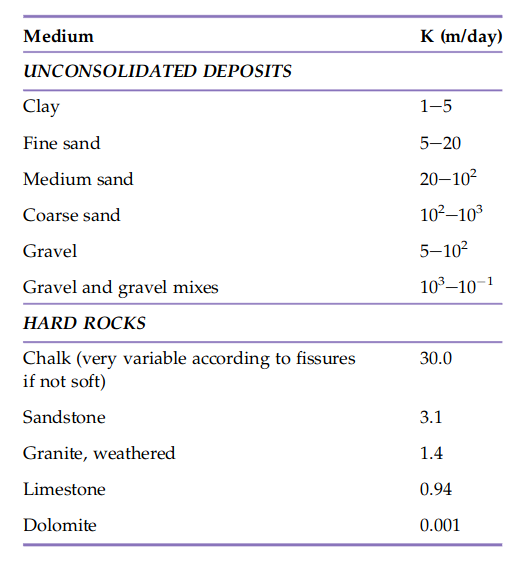
\includegraphics[scale=0.60]{Figura2.png}
\caption{Valores de conductividad hidráulica para varios tipos de sedimentos y roca consolidada (De Marsily,1986).}
\label{Figura2:1.2}
\end{figure}
\newpage

\section{Variabilidad espacial}

Los parámetros estudiados en la sección anterior se distribuyen de diferente forma en las formaciones geológicas, la carga hidráulica es un valor que se rige de forma deterministica a partir una ley física, mientras que la distribución de la conductividad hidráulica (suponiendo que el fluido de trabajo es el agua) depende principalmente de las propiedades del medio y de la geología de la zona por lo que el estudio de la variación de este parámetro se da esencialmente en términos estadísticos que son de vital importancia para conocer las rutas en las que viaja el flujo de agua.

\subsection{Homogeneidad y heterogeneidad}

La distribución de la conductividad hidráulica puede ser definida con un medio homógeneo, es decir, que el medio poroso esta configurado de tal forma que la conductividad hidráulica no varia en cada punto del mismo. La expresión que se ocupa para describir la homogeneidad, es la siguiente:

\begin{equation}
\label{eqn:phi11}
K(x,y,z)= C
\end{equation}

Donde K es una función de la posición del dominio (medio poroso) y C es una constante. En dado caso que K sea diferente a una constante y sea una función de la posición, nos encontramos con un material heterogéneo cuya conductividad esta espacialmente distribuida por $K(x,y,z)$.  
\\
\\
La heteregoneidad describe con mayor exactitud la complejidad de las formaciones geológicas que nos enfrentamos en la realidad. En el sentido estricto de la definición de homogeneidad, no existe formación alguna que tenga esas caracteristicas debido a que las formaciones geológicas son resultado de un conjunto de procesos geológicos que hacen imposible una homogeneización de sus componentes, por lo que para describir la heterogeneidad hay que tener en cuenta el ambiente geológico y cualquier combinación de estos. El tratamiento de la heterogeneidad en modelos de agua subterránea se pueden clasificar a partir del tipo de distribución de sus valores de conductividad y ajustar a modelos geológicos existentes.
\\
\\
El primer tipo de distribución de la heterogeneidad, es observada en el depósito intermitente de sedimentos que generan la estratificación en cuencas sedimentarias. En este tipo de estructuras geologicas existe una intercalación vertical de material geológico con diferentes valores de conductividad hidráulica, en cada capa se puede asumir un valor constante de conductividad hidráulica, sin embargo, el conjunto de bloques es un sistema heterogéneo. Un ambiente sedimentario donde exista una combinación de depósitos de alta energía con depósitos de baja energía ,generaría una secuencia de arcillas con arenas cuya composición genera una alta variación en la conductividad hidráulica, por lo que, combinado a la porosidad, la unidad de arenas es un potencial acuífero con barreras impermeables que representan las capas de arcillas. Un caso distinto es el causado debido a discontinuidades dentro de la formación debido a depósito reciente de sedimentos; en ambos casos, la configuración de la heterogeneidad es el punto de partida para definir la forma en la que se va a comportar el fluido en las formaciones geológicas. 
\\
\\ 
En el caso de ambientes sedimentarios donde existe una variación gradual del material a lo largo del espacio, se define otro tipo de distribución, una tendencia de heterogeneidad donde la conductividad hidráulica disminuye o aumenta dependiendo del proceso geológico que generó el ambiente sedimentario. Un ejemplo de esto ocurre en los depósito deltaicos, cuyo proceso de formación se basa en el transporte de sedimentos  en las desembocaduras fluviales donde se distribuye todo el sedimento en grandes áreas cerca y sobre el mar (Arche,2010). Al ser el agua del río el medio de transporte del sedimento, existe una mayor selección a lo largo de grandes tramos de viaje (mayor energía), por lo que las zonas más alejadas tienden a tener una conductividad más baja debido a los tamaños de grano más pequeños y mejor empaquetamiento, mientras que las zonas cercanas tienden a estar constituidas de gravas y arenas que tienden a tener una mayor conductividad hidráulica. Con esta distribución de materiales, la conductividad hidráulica puede variar en varios ordenes en cada dirección del delta. Otros ambientes geológicos que cuentan con una configuración de tendencia de heterogeneidad son ambientes de depósito glaciar o abanicos aluviales. También este tipo de heterogeneidad se puede encontrar en formaciones donde el movimiento del flujo se ve condicionado por fracturas y diaclasas \cite{Arche2010}. 

\begin{figure}[ht!]
\centering
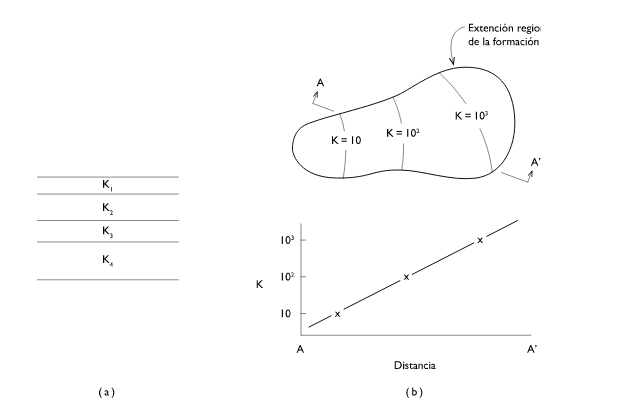
\includegraphics[scale=0.60]{Figura3.png}
\caption{Heterogeneidad en capas y en tendencia (Freeze and Cherry, 1979).}
\label{Figura2:1.3}
\end{figure}
La heterogeneidad en capas se ve representada en la figura \ref{Figura2:1.3}a, mientras que en la figura \ref{Figura2:1.3}b observamos un ambiente en planta cuya conductividad hidráulica varia en cualquier punto, donde tomando una dirección AA' la variación de la conductividad hidráulica es de 3 ordenes que puede variar en forma lineal como en la figura \ref{Figura2:1.3}b o tomar formas exponenciales o logaritmicas. Varios autores hacen la descripción de la heterogeneidad de un ambiente sedimentario a partir de las propiedades estadísticas del conjunto de valores de conductividad hidráulica, encontrando que la distribución de probabilidad que usalmente se encuentra en una formación geológica es log-normal (Freeze and Cherry, 1979; De Marsily, 1986), es decir, el logaritmo natural de la variable aleatoria que representa la distribución de la conductividad hidráulica nos proporciona una distribución de probabilidad normal también llamada gaussiana \cite{Freeze1979}\cite{Marsily1986}.

\begin{equation}
\label{eqn:phi12}
X=ln(K)
\end{equation}

Freeze (1975) hace un estudio de la conductividad hidráulica a partir de esta distribución, encontrando que la varianza usualmente se encuentra entre 0.15-1.5 dentro de una misma unidad geológica, por lo que incluso dentro de una formación que se supone homogénea existe una variación de entre 1 y 2 ordenes de magnitud respecto a la media. Incluso la heterogeneidad de tendencia puede entenderse como una distribución aleatoria donde existe una tendencia en el valor medio, por lo que existe un aumento en el valor de la tendencia media para el rango observado.
\\
\\
Es posible definir la heterogeneidad y la homogeneidad a partir de sus caracteristicas estadísticas. La homogeneidad de un medio es solo teórico, pero es posible aproximarlo como homogéneo si sus conductividades hidráulicas tienen una distribución unimodal, es decir, del conjunto de medidas de conductivades hidráulicas predomina un valor moda. Cuando por le contrario la conductividad hidráulica tiene una distribución multimodal, con más de dos valores moda, entonces se puede aproximar como heterogénea; como en el caso de la heterogeneidad de tendencia cuyo número de modas es el orden de variación de la conductividad hidráulica.
\\
\\
La definición clásica de homogeneidad también se puede describir estadísticamente como una distribución uniforme, por lo que en un sentido más estricto, al igual que la descarga específica, la conductividad hidráulica que se maneja usualmente es una conductividad hidráulica media de la formación geológica \cite{Freeze1979}.


\begin{figure}[htbp]
\centering
\subfigure[Unimodal]{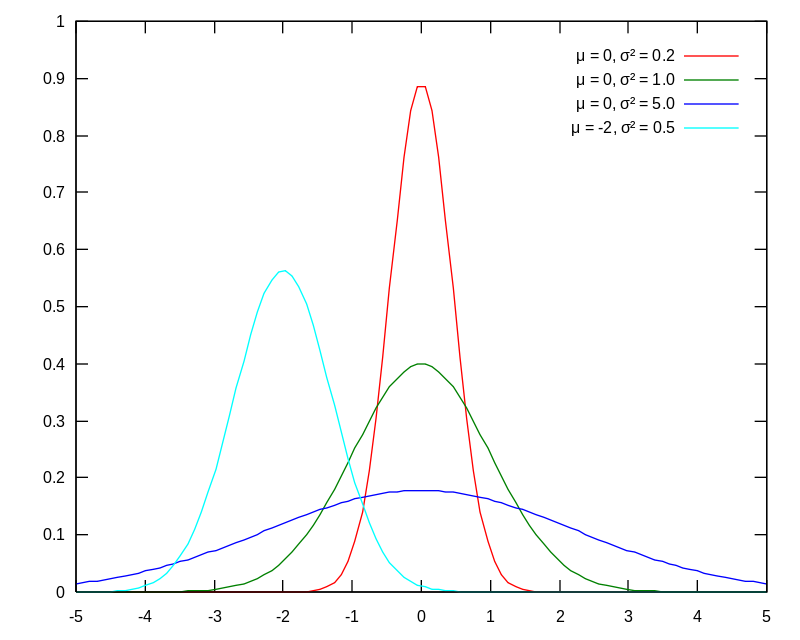
\includegraphics[width=40mm]{Figura5.png}}
\subfigure[Bimodal]{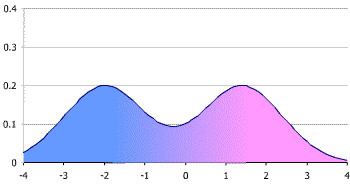
\includegraphics[width=40mm]{Figura4.png}}
\subfigure[Uniforme]{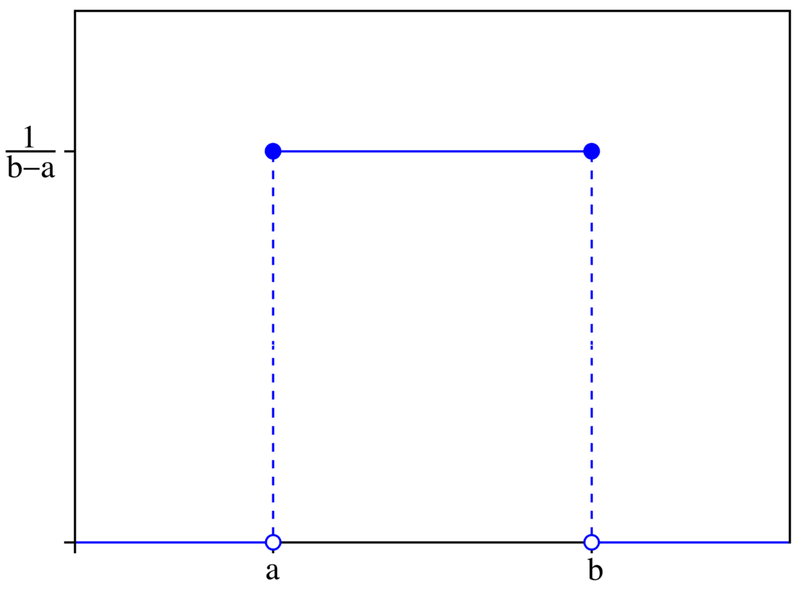
\includegraphics[width=80mm]{Figura6.png}}
\caption{Distribuciones de probabilidad de la conductividad hidráulica} \label{fig:lego}
\end{figure} 

\newpage

\subsection{Distribución geoestadistica de la heterogeneidad}

La variación espacial de la conductividad hidráulica necesita más herramientas para su análisis de las que proporciona la estadística univariada. Los principios básicos para estudiar la correlación que existe entre los valores de conductividad hidráulica o cualquier propiedad física del subsuelo con su posición espacial fue desarrollada por Matheron (1960) donde aplica las técnicas estudiadas por Krige(1941) para lo que asocia una variable aleatoria a cada punto del espacio. La rama de la estadística que estudia un conjunto de datos a partir de su variabilidad espacial se llama \emph{Geoestadística}, y tiene una amplia aplicación a fenómenos que se rigen por variables que son difíciles de modelar de forma determinista debido a que depende de procesos aleatorios \cite{Viera2002} \cite{Matheron1962} \cite{Krige1951}.
\\
\\
Para hacer la caracterización de la conductividad hidráulica a partir de la geoestadística, es necesario hacer un análisis de datos que consiste en determinar la influencia que se tienen respecto a su posición, por lo que a diferencia de la estadística clásica, las variables aleatorias que representan al fenómeno en un punto son dependientes a la variable aleatoria en otro punto, en otras palabras, existe correlación espacial entre variables aleatorias, por lo que es trabajo de la geoestadística determinar el grado y rango de influencia entre ellas, y a partir de este análisis ser capaz de hacer una predicción sobre su valor en cualquier posición de la zona de estudio.
\\
\\
La geoestadística trabaja principalmente con tres conceptos que definen al fenómeno que ocurre en la zona de estudio, en nuestro caso la conductividad hidráulica. La variable regionalizada es la primera a la que Matheron hace referencia, y se define como la variable distribuida en el espacio de manera que presenta una estructura espacial de correlación (Viera,2002). En casos prácticos, una variable espacial puede ser considerada como una variable regionalizada si se siguen las siguientes caracteristicas \cite{Rodriguez1999}\cite{Viera2002}.

\begin{itemize}
\item La variable espacial es continua pero no es posible de modelar de forma determinista. 
\item Exista variación local aleatoria.
\item Exista variación local no aleatoria.
\end{itemize}

Los ultimos dos puntos significan que la variable espacial puede tener un componente aleatorio y uno deterministico, aunque esta última es opcional pero su existencia nos da mas herramientas para su modelación
\\

La conductividad hidráulica en formaciones geológicas cumple con esas caracteristicas, donde la conductividad hidráulica para cada punto se representa por una variable aleatoria $K$, al conjunto de todas las variables aleatorias en cualquier punto del dominio se le conoce como función aleatoria y representa  al fenoméno en todo el dominio $K(x)$, esto significa conocer la conductividad hidráulica para cada punto del espacio, al nosotros poseer la información de $K$ sobre una zona en específico podemos obtener una muestra de $K(x)$ donde obtendriamos un fragmento de la variable regionalizada y un conjunto de valores discretos tales que $K'={K(x_{i}): x_{i}\in\Omega}$ ; donde esta muestra de la función aleatoria también se le conoce como \textbf{realización}.
\\
\\
La distribución espacial se puede estudiar a partir de un análisis estructural de los datos y obtener de esta forma los rangos de influencia que existen entre ellos, el \textbf{semivariograma} o \textbf{variograma} es la principal herramienta estadística que nos permite conocer esas características y hacer posteriormente un modelo de nuestra función aleatoria.
\\

Partimos de nuestra función aleatoria $K(x)$, a la que se le asume una función de semivarianza y se define de la siguiente forma:

\begin{equation}
\label{eq:Phi14a}
\gamma(h)=\dfrac{1}{2}Var[K(x)-K(x+h)]
\end{equation}

\begin{equation}
\label{eq:Phi14}
\gamma(h)=\dfrac{1}{2}E[{K(x)-K(x+h)}^{2}]
\end{equation}

Donde $h$ determina la magnitud del rango entre valores en dos puntos distintos y la dirección donde se realiza la medición, también conocido como lag.
\\
\\
Es imposible de conocer el valor de conductividad hidráulica para cada punto, por lo que el conjunto de muestras que conforman una realización son necesarias para hacer una estimación del semivariograma real, el estimador más común que se usa en la práctica es el siguiente:

\begin{equation}
\gamma(h)=\dfrac{1}{2N(h)}\sum_{i=1}^{N(h)}[K(x_{i}+h)-Z(x_{i})]^{2}
\end{equation}

Donde N(h) es el número de pares de puntos que existen en la variable regionalizada a una distancia $h$. El principal problema de este estimador recae en la selección de la muestra, es necesario que sea representativa de la función aleatoria para evitar semivariogramas erróneos, además, se debe de tomar los siguientes puntos a consideración para hacer una aproximación del semivariograma real \cite{Viera2002}

\begin{itemize}
\item Es recomendable trabajar con variables aleatorias de distribución normal. 
\item No debe de existir una relación entre la varianza y la magnitud del valor medio.
\item Evitar concentrar el muestreo en zonas de altos o bajos valores.
\item Tratar de evitar los outliers debido a problemas de medición.
\end{itemize}

Otros estimadores que se usan en la práctica son los estimadores de ponderación univariados y el estimador de Creesie y Hawkins (Viera,2002). 
\\
\\
Los semivariogramas muestrales que se producen en cualquier estimador, se clasifican en dos tipos principalmente, el primero consiste en que la semivarianza incrementa en función del aumento del intervalo $h$ hasta alcanzar un valor tope de semivarianza que se mantiene constante para cualquier $h$ de mayor valor, esto se interpreta como la distancia en la que los valores dejan de tener influencia entre ellos, estos son los variogramas transitivos donde el valor máximo es llamado \textbf{sill} mientras que la distancia máxima de afectación es llamado \textbf{rango}.

\begin{figure}[ht!]
\centering
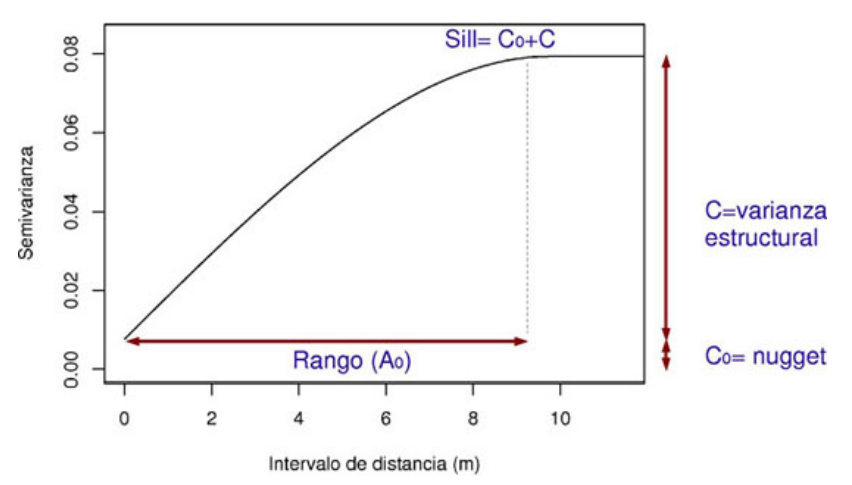
\includegraphics[scale=0.50]{Figura7.jpeg}
\caption{Elementos de un variograma transitivo (Gallardo, 2009)}
\label{Figura6:1.6}
\end{figure}

El segundo tipo de semivariograma muestral es cuando no existe sill ni rango, es decir, la curva crece con valores de semivarianzas infinitas a rangos infinitos, por lo que un punto cualquiera se ve afectado por otro aunque la distancia $h{\to}inf$, un aspecto que tienen ambos tipos de semivariogramas es la posible existencia del efecto \textbf{nugget} que se ve representado como la intersección en el eje de semivarianzas de la curva del semivariograma, contrario a la definición de semivariograma teórico donde se cumple que $\gamma(0)=0$; matematicamente esto simboliza una discontinuidad en la función aleatoria, pero en la práctica es debido a la escala del muestreo y a los errores comunes de medición.
\\
\\
Los datos que se obtienen en la práctica deben de ser ajustados a un semivariograma teórico a partir del semivariograma muestral para hacer uso de sus propiedades y poder realizar estimaciones o simulaciones de su distribución espacial, para ello se ocupan las características de rango, sill y nugget, no todos los modelos teóricos pueden ser utilizados para este propósito, deben de cumplir ciertas especificaciones dadas por un estudio de su transformada de fourier. Los principales semivariogramas teóricos ocupados en la práctica se dividen de igual forma en transitivos y no acotados, en esta tesis, la descripción de la heterogeneidad aleatoria se hará a partir de una distribución basada en un modelo teórico transitivo, por lo que seran los estudiados en esta sección.
\\
\\
El modelo lineal consiste en una zona de transición donde la variación del intervalo con la semivariacia es lineal hasta el rango donde el sill se mantiene constante, la función del semivariograma lineal se expresa de la siguiente forma:

\begin{equation}
\gamma(h)= \left\{ \begin{array}{lcc}
             S(h/a) \quad  para  \quad 0 \leq x \leq a \\
             \\ S \quad para \quad 2h>a  
             \end{array}
   \right.
\end{equation}

El modelo esférico consiste en la zona de transición como la intersección de dos esferas de diamétro a y distancia de sus centros d. Es un método apropiado principalmente para el caso de tres dimensiones aunque es posible usarse para una o dos , la expresión que determina su variograma es el siguiente:

\begin{equation}
\gamma(h)= \left\{ \begin{array}{lcc}
             \dfrac{S}{2}(3(\dfrac{h}{a})-\dfrac{h}{a}^{3})) \quad para \quad 0 \leq h \leq a \\
             \\ S \quad  para \quad 2  h > a  
             \end{array}
   \right.
\end{equation}

El modelo exponencial es más ocupado debido a la gran cantidad de fenoménos físicos que se rigen de esta forma, su zona de transición crece de forma exponencial mientras que la semivariancia tiende al sill cuando $h\rightarrow\inf$, la función queda determinada de la siguiente forma:

\begin{equation}
\gamma(h)=1-e^{\dfrac{-3h}{a}} \quad para \quad h>=0
\end{equation}

El modelo gaussiano, al igual que el exponencial, alcanza el sill de forma asintotica por lo que el rango es definido cuando el intervalo $h$ alcanza hasta un 95 por ciento del sill.

\begin{equation}
\gamma(h)=1-e^{\dfrac{-3h^{2}}{a^{2}}} \quad para \quad h >= 0    
\end{equation}

Los datos que obtenemos en el semivariograma muestral se ajustan a un modelo teórico a partir de métodos de ajuste, tales como minimos cuadrados, minimos cuadrados generalizados o minimos cuadrados ponderados, de esta forma tenemos una representación de nuestra variable regionalizada caracterizada por un variograma teórico que busca representar con mejor exactitud la variabilidad espacial de nuestro fenómeno. Este paso es fundamental para distribuir espacialmente nuestra conductividad hidráulica conociendo la estructura de nuestros datos \cite{Gallardo2006}.

\begin{figure}[htbp]
\centering
\subfigure[]{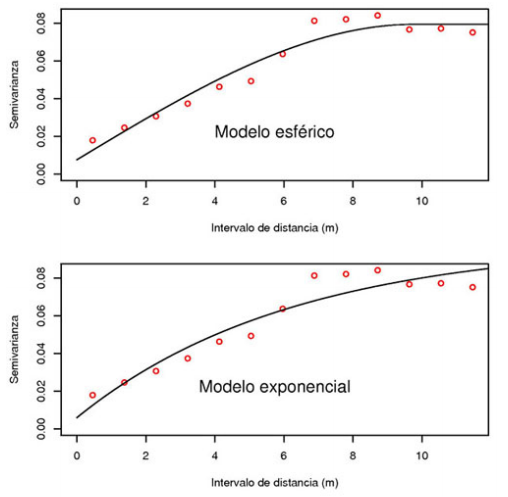
\includegraphics[width=70mm]{Figura12.png}}
\subfigure[]{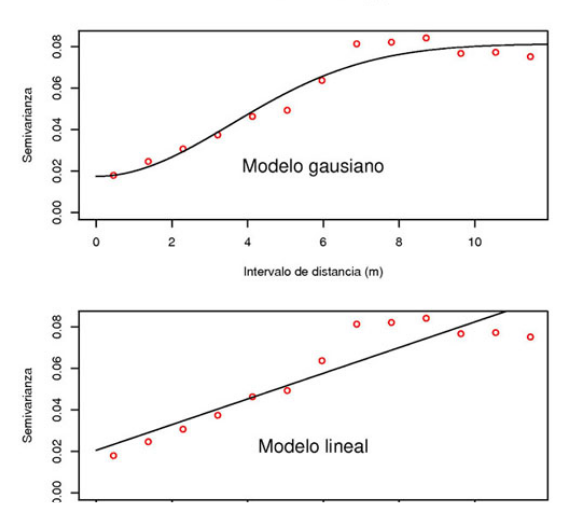
\includegraphics[width=75mm]{Figura11.png}}
\caption{Modelos de semivariogramas teóricos (Gallardo, 2006).} \label{fig:lego}
\end{figure} 

\section{La ecuación de flujo }

Según lo visto en secciones anteriores, el flujo de agua subterránea ocurre debido a procesos físicos que pueden ser modelados a partir de una ecuación matemática y asi definir la carga hidráulica en cada punto del dominio. Para poder definir la red de flujo es necesario combinar la ecuación de Darcy, ley empírica resultado de un balance de fuerzas, con la ecuación de continuidad, un balance de masa que garantiza la existencia del flujo másico a través de una porción elemental de medio poroso; el resultado de esta combinación da como resultado una ecuación diferencial parcial cuya solución es la carga hidráulica y su gradiente los patrones de flujo.
\\
\\
Para obtener la ecuación de continuidad para medios porosos, tomaremos un volumen elemental de dimensiones $\Delta{x}$, $\Delta{y}$ y $\Delta{z}$ donde el flujo másico se introduce de forma normal a cada una de las caras del volumen elemental, por lo que el flujo masico antes de atravesar la porción de medio poroso queda expresada como $\rho{\textbf{q}}\Delta{n}$, donde $\rho$ es la densidad del fluido con unidades (m/v), $\textbf{q}$ es el vector de descarga especifica con unidades (l/t) y $n$ representa el área de la cara donde el flujo incide normalmente en la dirección de $\textbf{q}$, el flujo másico después de atravesar el medio poroso debe permanecer invariable según la ley de conservación de masa, por lo que el flujo másico en la salida se ve expresada por la expresión inicial más la variación del flujo de masa por unidad de área del volumen elemental  ($\rho\textbf{q}$) respecto a la dirección de $\textbf{q}$ por la longitud del tramo de viaje. La ecuación de continuidad se ve expresada en la figura \ref{Figura6:1.6} en un sistema coordenado $xyz$.

\begin{figure}[ht!]
\centering
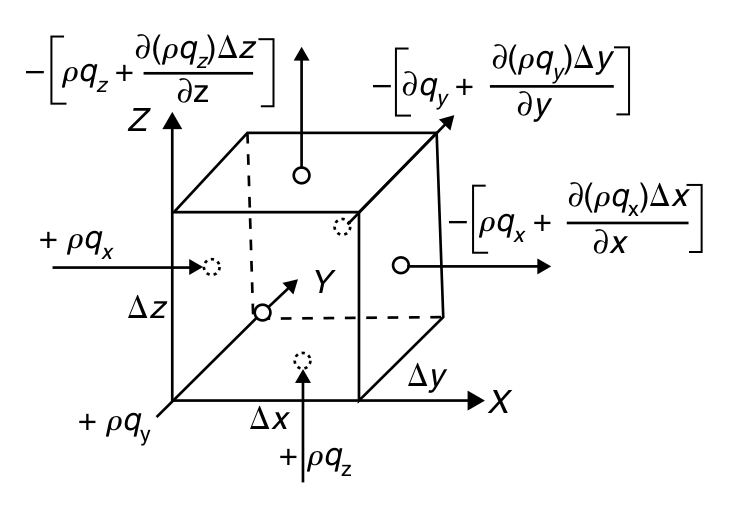
\includegraphics[scale=0.50]{Figura13.png}
\caption{Volumen elemental en ecuación de continuidad (Toth,2009).}
\label{Figura6:1.6}
\end{figure} 

El balance de flujo másico en cada dirección se ve expresada de la siguiente forma:

\begin{equation}
\label{eqn:Phi15}
\rho{q_{x}}\Delta{y}\Delta{z}-(pq_{x}+\dfrac{\partial{\rho{q_{x}}}}{\partial{x}})\Delta{x})\Delta{z}\Delta{y} 
\end{equation} 

\begin{equation}
\label{eqn:Phi16}
\rho{q_{y}}\Delta{z}\Delta{x}-(pq_{y}+\dfrac{\partial{(\rho{q_{y}})}}{\partial{y}})\Delta{y})\Delta{z}\Delta{x}  
\end{equation}

\begin{equation}
\label{eqn:Phi17}
\rho{q_{z}}\Delta{y}\Delta{x}-(pq_{z}+\dfrac{\partial{\rho{q_{z}}}}{\partial{z}})\Delta{z})\Delta{x}\Delta{y}  
\end{equation}  

Cancelando los términos similares y suponiendo que no existen fuentes externas que aporten al flujo másico, la variación del flujo sera igual a cero $\Delta{\dot{m}=0}$ y quedará expresada en función de la varación del flujo másico, por lo que la ecuación de continuidad queda de la siguiente forma:

\begin{equation}
\label{eqn:Phi17}
\Delta{x}\Delta{y}\Delta{z}[\dfrac{\partial(\rho{q_{x}})}{\partial{x}}+\dfrac{\partial(\rho{q_{y}})}{\partial{y}}+\dfrac{\partial(\rho{q_{z}})}{\partial{z}}]=0
\end{equation} 

\begin{equation}
\label{eqn:phi18}
\bigtriangledown(\rho\textbf{q})=0
\end{equation}

La parte interna del lado derecho de la ecuación \ref{eqn:Phi17} se puede desarrollar a partir de la regla para derivación de productos, suponiendo que el agua es el fluido de trabajo y tiene la caracteristica de tener una densidad constante ($\rho=cte$) , la ecuación final queda de la siguiente forma:

\begin{equation}
\label{eqn:phi19}                                                             \rho[\dfrac{\partial(q_{x})}{\partial{x}}+\dfrac{\partial(q_{y})}{\partial{y}}+\dfrac{\partial(q_{z})}{\partial{z}}]+\textbf{q}[\dfrac{\partial{\rho}}{\partial{x}}+\dfrac{\partial{\rho}}{\partial{y}}+\dfrac{\partial{\rho}}{\partial{z}}]=0
\end{equation}

\begin{equation}
\label{eqn:phi20}     \dfrac{\partial{(q_{x})}}{\partial{x}}+\dfrac{\partial{(q_{y})}}{\partial{y}}+\dfrac{\partial(q_{z})}{\partial{z}}=0
\end{equation}

\begin{equation}
\label{eqn:phi21}
\bigtriangledown(q)=0
\end{equation}

Donde la ecuación \ref{eqn:phi20} es la ecuación de continuidad para fluidos ligeramente compresibles, para concluir el modelo matemático es necesario introducir la ley de Darcy que representa el comportamiento del fluido cuando viaja en un medio poroso.

\begin{equation}
\label{eqn:phi22}
q_{x}=-K_{x}\dfrac{\partial{h}}{\partial{z}}
\end{equation}

\begin{equation}
\label{eqn:phi23}                          q_{y}=-K_{y}\dfrac{\partial{h}}{\partial{y}}
\end{equation}

\begin{equation}
\label{eqn:phi24}                         q_{z}=-K_{z}\dfrac{\partial{h}}{\partial{z}}
\end{equation}

Combinando las ecuaciones de Darcy y de continuidad, obtenemos la ecuación diferencial que representa al fenoméno del flujo de agua subterránea en medios porosos en función de la carga hidráulica.

\begin{equation}
\label{eqn:phi25}                         
\dfrac{\partial}{\partial{x}}(Kx\dfrac{\partial{h}}{\partial{x}})+\dfrac{\partial}{\partial{y}}(Ky\dfrac{\partial{h})}{\partial{y}}+\dfrac{\partial}{\partial{z}}(Kz\dfrac{\partial{h}}{\partial{z}})=0
\end{equation}

La expresión \ref{eqn:phi25} es llamada ecuación de Laplace para medios anisotrópicos y heterogéneos, para casos donde el dominio es homogéneo e isotrópo, la expresión se reduce de la siguiente forma:

\begin{equation}
\label{eqn:phi26}
\dfrac{\partial^{2}h}{\partial{x^{2}}}+\dfrac{\partial^{2}h}{\partial{y^{2}}}+\dfrac{\partial{^{2}h}}{\partial{z^{2}}}=0
\end{equation}

\begin{equation}
\label{eqn:phi27}
\bigtriangledown^{2}(h)=0
\end{equation}

La ecuación \ref{eqn:phi27} también se puede definir para un medio isotrópico pero heterogéneo, donde la conductividad hidraúlica es una función aleatoria que reproduce en exactitud la variación espacial en todo el dominio.

\begin{equation}
\label{eqn:phi28}                         
\dfrac{\partial}{\partial{x}}(K(\textbf{x})\dfrac{\partial{h}}{\partial{x}})+\dfrac{\partial}{\partial{y}}(K(\textbf{x})\dfrac{\partial{h}}{\partial{y}})+\dfrac{\partial}{\partial{z}}(K(\textbf{x})\dfrac{\partial{h}}{\partial{z}})=0
\end{equation}

Donde \textbf{x} es una variable aleatoria para cada punto de coordenadas ${x,y,z}$. En dado caso que exista alguna fuente como la existencia de un pozo de extracción o absorción, se puede expresar con una función $f(x,y,z)$ en el lado derecho de la ecuación \ref{eqn:phi20}, la ecuación modificada es llamada ecuación de poisson:
 
 \begin{equation}
\label{eqn:phi29}                         
\dfrac{\partial}{\partial{x}}(K(\textbf{x})\dfrac{\partial{h}}{\partial{x}})+\dfrac{\partial}{\partial{y}}(K(\textbf{x})\dfrac{\partial{h})}{\partial{y}}+\dfrac{\partial}{\partial{z}}(K(\textbf{x})\dfrac{\partial{h}}{\partial{z}})=f(x,y,z)
\end{equation}

Existen dos formas diferentes de resolver ecuaciones diferenciales, la primera es obtener una solución analitica que se cumpla para todo dominio y que cumpla las condiciones de frontera, sin embargo, estas soluciones de $h$ obligan a simplificar el problema hasta un modelo que dista mucho de la complejidad del medio poroso, por lo que generalmente se ocupan métodos númericos para obtener soluciones aproximadas que puedan acercarse lo más posible a la solución exacta \cite{Toth2009} \cite{Freeze1979}.
